%%%% ijcai15.tex

\typeout{IJCAI-15 Instructions for Authors}

% These are the instructions for authors for IJCAI-15.
% They are the same as the ones for IJCAI-11 with superficical wording
%   changes only.

\documentclass{article}
% The file ijcai15.sty is the style file for IJCAI-15 (same as ijcai07.sty).
\usepackage{ijcai15}

% Use the postscript times font!
\usepackage{times}

\usepackage[pdftex]{graphicx}
%\usepackage{cite}
%\usepackage[cmex10]{amsmath}
%\usepackage{algorithmic}
%\usepackage{url}
%\usepackage{mdwmath}
%\usepackage{mdwtab}


% the following package is optional:
\usepackage{latexsym} 

% Following comment is from ijcai97-submit.tex:
% The preparation of these files was supported by Schlumberger Palo Alto
% Research, AT\&T Bell Laboratories, and Morgan Kaufmann Publishers.
% Shirley Jowell, of Morgan Kaufmann Publishers, and Peter F.
% Patel-Schneider, of AT\&T Bell Laboratories collaborated on their
% preparation.

% These instructions can be modified and used in other conferences as long
% as credit to the authors and supporting agencies is retained, this notice
% is not changed, and further modification or reuse is not restricted.
% Neither Shirley Jowell nor Peter F. Patel-Schneider can be listed as
% contacts for providing assistance without their prior permission.

% To use for other conferences, change references to files and the
% conference appropriate and use other authors, contacts, publishers, and
% organizations.
% Also change the deadline and address for returning papers and the length and
% page charge instructions.
% Put where the files are available in the appropriate places.

\title{Energy Aggregation using Product of Experts\thanks{These match the formatting instructions of IJCAI-07. The support of IJCAI, Inc. is acknowledged.}}
\author{Megha Gupta 
%Dept. of Computer Science, IIIT Delhi\\
\texttt{meghag@iiitd.ac.in}\\
Haimonti Dutta
%Department of Management Science and Systems,\\%
%State University of New York, Buffalo\\ New York, 14260\\
\texttt{haimonti@buffalo.edu}\\
Amarjeet Singh
%Dept. of Computer Science, IIIT Delhi\\
\texttt{amarjeet@iiitd.ac.in}\\
Ullas Nambiar
%EMC Corporation,\\
%Bangalore, India\\
\texttt{Ullas.Nambiar@emc.com}
}

\begin{document}

\maketitle

\begin{abstract}
%  The {\it IJCAI--15 Proceedings} will be printed from electronic
%  manuscripts submitted by the authors. The electronic manuscript will
%  also be included in the online version of the proceedings. This paper
%  provides the style instructions.
\end{abstract}

\section{Introduction}

%The {\it IJCAI--15 Proceedings} will be printed from electronic
%manuscripts submitted by the authors. These must be PDF ({\em Portable
%Document Format}) files formatted for 8-1/2$''$ $\times$ 11$''$ paper.

Smart meters consisting of real time sensors, power outage notifications and power quality monitoring are widely used today. These meters provide a host of benefits like energy efficiency and savings, improved retail competition, better demand response actions, improved tariffs, lower bills due to better customer feedback, accurate billing, less environmental pollution, etc. %\cite
They generate huge amount of data which helps in giving meaningful insights through analytics.
They can measure site specific information and also help agencies to set different electricity prices for consumption based on the time of the day, seasons, holidays, etc. As a result, a feedback is sent to the customers by the utilities that can help consumers better manage their resources. A research \cite{mckerracher} shows that by providing real time feedback, consumers can reduce the consumption by 3-5\%. Also, for some country providing real time feedback may not be a cost effective plan but it can help in retaining customers and peak-load shift.
%This helps consumers to better manage their energy resources and reduce their bills and carbon emissions.


In recent years, machine learning has been applied to the problem of energy consumption and demand forecasting analysis. The role of the machine learning algorithm is to study the sensor data and provide alerts and warnings when anomalous behaviour occurs or to inform (and remind) customers when certain activities were performed, which rooms they occupied, and what appliances they used most frequently during that period. This information can be transmitted to customers in timely fashion via phone, email or the Internet.
This paper \cite{1626400} does a comparison of several clustering techniques and finds out that  the hierarchical clustering and modified follow-the-leader perform best among the rest K-Means, fuzzy K-Means to group customers with similar electrical behaviour \cite{5620917}. Another paper \cite{Wijaya} uses classifiers like random forest, J48, logistic and naive bayes to identify customers with similar electricity consumption profiles.
Sensor data collected from smart homes are used to reveal activity patterns of the residents, which can then be correlated with the total energy consumption. This enables utility companies and their customers to associate activities with energy usage and costs, devise intelligent systems to control home environments improving energy efficiency and reducing costs. Typically, sequences of usage patterns that appear frequently at different time scales (daily, weekly, monthly, yearly) and across different homes are studied and 
%; trends of electricity consumption (steadily increasing, decreasing, cyclic, seasonal) for individual homes and across the community; and anomalies (sudden peaks or drops on consumption) for individual homes and across the community.
outlier detection algorithms are designed to enable customers to be notified that they are consuming unusually large amount(s) of energy during some specific period. Related problems involve study of trends of electricity consumption (steadily increasing, decreasing, cyclic, seasonal) and sudden anomalous behaviour (sudden peaks or drops on consumption) for individual homes and across the community.

In this paper, we build machine learning models using products of HMM and apply them to the energy aggregation problem. Two different proof of concepts are presented -- one on the REDD data set and another on real data collected at the faculty housing in India. 
%application of are aggregating energy consumption information using a model that extends the power of HMMs. HMM's are used as the basic expert in the of product of experts model. 
There are many reasons why the product model constructed from many HMMs is appropriate. First, this model is ideal for data which is caused by multiple underlying influences. Second, HMMs alone are not efficient at capturing long range structure in time series \cite{Taylor} -- in contrast to product of hidden markov models (PoHMM)  \cite{andrew} allow each model to remember a different piece of information about the past.
%There have been some experiments on sentence and character strings modelling, factorial time series to demonstrate the advantages of using a PoHMM over an equivalently sized regular HMM}.
%We have applied the contrastive divergence learning algorithm on two datasets, REDD dataset and the faculty housing dataset which was generated by smart meters.
%The system architecture for the faculty housing dataset consists of two smart meters $S_1$ and $S_2$ installed in a faculty housing building collecting data from twelve floors. $S_1$ collects data from first six floors (0 to 5th) and $S_2$ collects data from the rest of the floors (6 to 11th). The data collected from two meters is aggregated using product of experts technique in a way that the contrastive divergence between the two probability distributions is minimized. 
%The proof of concept of REDD dataset and faculty housing dataset is given in section~\ref{sec:redd} and section~\ref{sec:faculty} respectively.

\noindent \textbf{Organization:} This paper is organized as follows: Section~\ref{related} examines related work on data analytics on aggregated data of smart meters; Section~\ref{sec:review} provides a review of products of Hidden Markov Models (HMMs) and how they relate to our application. The two proofs of concepts are introduced in Section~\ref{poc} to illustrate the effectiveness of the use of product of HMMs in the energy aggregation problem. Finally, Section~\ref{conc} concludes the work.

\section{Related Work}
\label{related}
In this section, we describe work that uses ensemble learning techniques and non-ensemble learning techniques to solve problems in energy domain.
\subsection{Non-ensemble based learning techniques}

\subsubsection{Energy Aggregation}
%Devaine et al. (CITE) study ...
In wireless sensor networks, energy data aggregation is a method of combining data from different sources and expressing on a specific variable, in a summarised format. As the sensor network generates lot of data for the end user to process, there are automated methods employed to aggregate data. This data fusion is generally known as data aggregation which combines the data into a set of meaningful information \cite{Heinzelman00energy}.
The sensor nodes are organised in a tree structure, called aggregation tree. The leaves of this tree are the sensor devices, the internal nodes are the aggregator devices that takes the data from the leaves, aggregates it and sends it to its parent node which is the root of the tree. \\
The main objective of data aggregation is to reduce the unnecessary information thereby reducing the network traffic and improving the privacy of the customers from internal and external entities by keeping only the necessary information \cite{taban}. 


%To study the process of energy aggregation, data is collected from multiple smart meters. This collected data is very large which in turn makes the analytics on top of it very difficult. Also, this detailed energy consumption data leads to privacy breach and other risks related to it. To address this problem, there has been work done \cite{Wijaya} to reduce the smart meter data numerosity by converting it into symbolic representation and then allowing algorithms on top of it. They have applied the symbolic representation tasks for customer segmentation and load forecasting.

%The purpose of energy aggregation is to get some valuable information about single or multi-site units. 
%This work evaluates the trend of degrading performance of the state of the art algorithms when the number of considered meters decrease \cite{BLTJ:BLTJ21650}. Short term load forecasts at the meter level help the company communicate with the customer about energy savings and billing. STLF handles prediction of one hour upto one week.
%The energy aggregation problem has been tackled in a variety of ways including topology control, energy conserving sleep scheduling, mobile data collectors and data aggregation. 
%Research has been done on the role of energy on the growth of the country's economy \cite{NYAS:NYAS5921}.

\subsubsection{Energy Disaggregation}
The process in which the whole building energy (aggregated) signal is separated into appliance level energy (disaggregated) for a variety of reasons like residential energy reductions, program evaluation, targeted marketing, etc. Several studies have been done in this regard, one of the unsupervised desegregation method \cite{DisaggregationHSMM} that outperforms other unsupervised disaggregation methods is conditional factorial hidden semi-Markov model. This model when integrated with other features, accurately represents the individual appliance energy consumption. Another research \cite{KolterJ12} that exploits the additive structure of the FHMM to develop approximate inference procedure in  energy disaggregation domain that outperforms the rest.

\subsubsection{Load Forecasting}
Electrical load forecasting refers to the projection of electrical load required in a certain geographical area with the use of previous electrical load usage in the same area. It is extremely important for efficient power system planning and operation, energy purchasing and generation, load switching, infrastructure development. It encompasses various factors like, historical load, weather data, population, energy supply and price, time of the year, etc.
It is usually divided into three categories, short-term forecasts (one hour to one week) , medium-term forecasts (one week to one year) and long-term forecasts (more than a year).
In short term load forecast, \cite{Bakirtzis} and \cite{Chen} used a three layer feed forward artificial neural network and to predict daily load profiles. In a paper by \cite{Chow}, nonlinear autoregressive integrated neural network was used to predict daily load consumption.
In medium term load forecasts, the author forecasts \cite{Falvo} the monthly load through knowledge based activities from the output of the ANN based stage providing yearly energy predictions. Whereas in \cite{bassi}, time lagged feedforward neural network is used to do monthly forecasting on the basis of historical series of electrical load, economic and demographic variables. And the authors from covenant university, \cite{samuel} performed load forecasting of their own educational institute using the models based on linear, compound growth and cubic methods of regression analysis.
In long term load forecasting, study done by \cite{Daneshi} resulted in showing that the models based on regression analysis did not give very accurate predictions as compared to fuzzy neural network which performed better due to better handling with non linear systems. Another work  \cite{Zhang} uses support vector regression to derive non linear relationship between load and economic factors like GDP for long term forecasting in developing countries.



\subsubsection{Customer Segmentation}
The identification of consumer profiles that show similar behaviour in energy consumption. This analysis is useful in various ways, like demand response system, intelligent distribution channel. The author \cite{wijaya2014consumer} segments the customers based on contextual dimensions like location, seasons, weather patterns, holidays, etc which help with various higher level applications like usage-specific tariff structure, theft detection, etc. In \cite{Albert}, author proposes to infer occupancy states from consumption time series data by using HMM framework. They investigate the effectiveness of HMM and model based cluster analysis in producing meaningful features of the classification. This work suggests the dynamics of time series as captured by HMM analysis can be valuable.

\subsection{Ensemble based learning techniques}
Ensemble learning is a method where multiple learners are trained to solve the same problem. It constructs a set of hypothesis and combines them to generate the final result.
\subsubsection{Prediction with expert advice}
A study done by \cite{Shen}, proposes a Pattern Forecasting Ensemble Model (PFEM) comprising of five forecasting models using different clustering techniques, like k-means model, self-organising map model, hierarchical clustering model, k-medoids model and fuzzy c-means model. They have showed that on three real-world dataset, their proposed ensemble model outperformed all the five individual model in case of day ahead electricity demand prediction.
Another study \cite{Felice} highlights the importance of regularised negative correlation learning ensemble methodology on the problem of energy load hourly prediction. This method tries to overcomes the problem of variability in neural network due to high sensitivitiness to the initial conditions. As this method combines the outputs of several neural networks, it achieves a marked reduction in error after introducing external data. \\
In our paper,  we deal with the problem of energy aggregation using ensemble learning model. Each HMM is used to represent a state of an appliance. An appliance can have states like ON or OFF. The combination of the outputs from each of these HMM models gives us our ensemble based learning model, Product of Hidden Markov Model (PoHMM) \cite{hinton2000}. This learning technique outputs the probability distribution by combining the outputs from several simpler distributions. It allows each model to make a decision on the basis of few dimensions.


\section{Review of PoHMM}
\label{sec:review}
%Benveniste defines HMM as a triple (\'{A}, $\mu$, $\pi$) where \'{A} = (X,$X_0$,A,T) is an automaton, $\mu$ is the initial state probability, $\pi$ is factored as state transition probability $\pi$$_{x}$ and message transition probability $\pi$$_{A}$. He uses a random arbiter $\alpha$, with values {first, second, third} to choose automaton to initiate transition. If $\alpha$ = first then first automaton chooses any transition having a private message whereas second automaton performs a stuttering transition, and vice versa for $\alpha$ = second. If $\alpha$ = both, then both automata agree on some shared message and move accordingly.

Using the traditional HMM notation of the parameters $\lambda$ = \{A, B, $\pi$ \} where A is the transition probability, B is the observed probability, $\pi$ is the initial state probability. For a HMM, R we have the values of A, B, $\pi$ as shown in table ~\ref{table:A}, ~\ref{table:B}, ~\ref{table:pi} respectively.

%Distributed networks can be modeled using interacting automata.
%Benveniste \cite{benveniste} defines automaton as a quadruple, \'{A} = (X,$X_0$,A,T) where X is a finite state of sets, $X_0$ is the subset of initial states, A is a finite set of messages, T is a set of transitions of the form t = \{x\_,a,x\} where x\_ is the previous state, a is the message label on which the state transitions to the next state x. The figure~\ref{fig:ex} below explains the automata with an example.\\

\begin{figure*}[t]
\centering
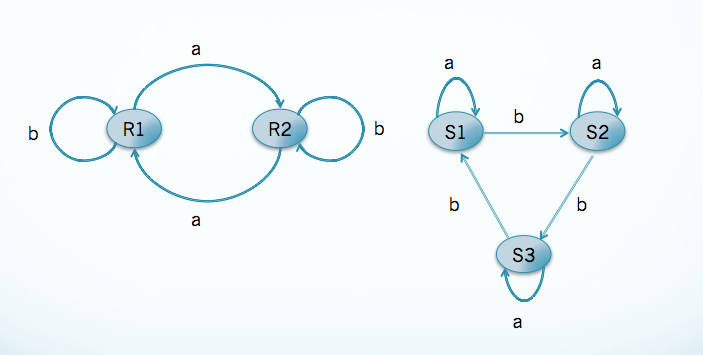
\includegraphics[width=8cm,height=3cm]{automata.png}
\caption{HMM R and S}
\label{fig:ex}
\end{figure*}

For HMM R, X$_{R}$ = \{2; $R_1$,$R_2$\}, X$_{0R}$ = \{$R_1$\}, A$_{R}$ = \{a,b\}, T$_{R}$ = \{$R_1$,a,$R_1$; $R_1$,b,$R_2$; $R_2$,a,$R_2$; $R_2$,b,$R_1$\} \\
For HMM S, X$_{S}$ = \{3; $S_1$,$S_2$,$S_3$\}, X$_{0S}$ = \{$S_1$\}, A$_{S}$ = \{a,b\}, T$_{S}$ = \{$S_1$,a,$S_1$; $S_1$,b,$S_2$; $S_2$,a,$S_2$; $S_2$,b,$S_3$; $S_3$,a,$S_3$; $S_3$,b,$S_1$\} \\
The product of two automata \'{A} = R x S is defined as follows: \\
X = X$_{R}$ x X$_{S}$ \\
$X_0$ = X$_{0R}$ x X$_{0S}$ \\
A = A$_{R}$ $\cup$ A$_{S}$ \\
%t = (x\_,a,x)  \\

%Benveniste uses a notion of stuttering transition which helps to distinguish between local and global time by inserting dummy transitions between two transitions of a local automaton attached to a node. This stuttering transition waits for others to progress.

\begin{table}[h]
\centering
\begin{tabular}{ l | c | c }
 A & $R_1$ & $R_2$ \\
\hline
$R_1$ & 0.6 & 0.4 \\
$R_2$ & 0.3 & 0.7 \\
\end{tabular}
\caption{Transition probability, A}
\label{table:A}
\end{table}

\begin{table}[h]
\centering
\begin{tabular}{ l | c | c }
 B & a & b \\
\hline
$R_1$ & 0.2 & 0.8 \\
$R_2$ & 0.5 & 0.5 \\
\end{tabular}
\caption{Observed probability, B}
\label{table:B}
\end{table}

\begin{table}[h]
\centering
\begin{tabular}{ l | c | c }
&  $R_1$ & $R_2$ \\
\hline
$\pi$ & 0.4 & 0.6 \\

\end{tabular}
\caption{Initial state probability, $\pi$}
\label{table:pi}
\end{table}

%Talking in terms of HMM, requires us to equip products of automata with probabilities. 

\subsection{Product of HMM}
\label {sec:pohmm}
PoHMM is a combination of directed and undirected graphical models. The hidden states are connected with directed links where as the connection with visible states is through undirected links. This causes different conditional independence relationships among the variables in graphical model. 
Product of HMM is a way of combining HMM's to form distributed state time series model. It is defined by multiplying together the densities of its, k experts and renormalizing them. The figure~\ref{fig:pohmm} is a product of two HMMs shown in~\ref{fig:ex}. For  P = R x S, the quadruple becomes\\
X = \{6; $R_1$$S_1$, $R_1$$S_2$, $R_1$$S_3$, $R_2$$S_1$, $R_2$$S_2$, $R_2$$S_3$\} \\
$X_0$ = \{$R_1$$S_1$\} \\
A = \{a,b\} \\
%The rules for synchronised product construction are : \\
%1. $<p,q>$ --a--$>$ $<p',q>$ if a $\in$ A$_{R}$ $\cap$ A$_{S}$ and p --a--$>$ p' and q --a--$>$ q'	\\
%2. $<p,q>$ --a--$>$ $<p',q>$ if a $\in$ A$_{R}$, a $\notin$ A$_{S}$ and p --a--$>$ p'	\\
%3. $<p,q>$ --a--$>$ $<p,q'>$ if a $\notin$ A$_{R}$, a $\in$ A$_{S}$ and q --a--$>$ q'	\\

\begin{figure*}[t]
\centering
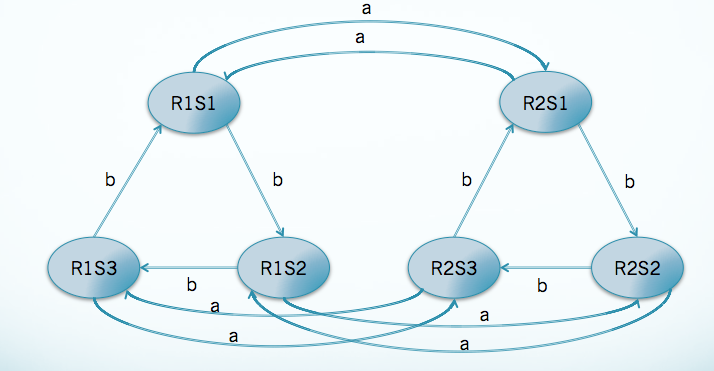
\includegraphics[width=8cm,height=3cm]{product.png}
\caption{Product of HMMs, P = R x S}
\label{fig:pohmm}
\end{figure*}

%\section{ Methodology }
%\label{sec:method}
\subsection{Inference in PoHMM}
The main feature of PoE is its undirected graphical modelling with no direct connection among the latent variables as they only interact indirectly via observed variables. The hidden variables all the experts are rendered independent when conditioned on visible variables. So, if the inference in each of the constituent model is tractable then the inference in the product is also tractable. To generate a data point in this model, all the experts in PoE generate an observation and if they all generated the same point then it is accepted else they again generate an observation until all the experts agree to it. Therefore all the experts have some influence over the generated data. So, the inference determines the the probability that all the experts would have taken in order to generate the given observation. 
 
\subsection{Training product of experts by minimising contrastive divergence}
PoE is a method of combining densities of many latent variable models. It is defined by the following formula:\\
% Write the formula and explain it. Explain Gibbs Sampling
To fit the model to the data, we need to maximize the likelihood of the dataset or minimise the Kullback-Liebler divergence between the real data and the fantasy data. The contrastive divergence algorithm for training the PoHMM has the following steps:
\begin{enumerate}
\item Calculate each model's gradient on a data point using forward backward algorithm.
\item For each model take a sample from the posterior distribution of paths through state space.
\item At each time step, multiply together the distributions and renormalize to get the reconstruction distribution at each step.
\item Draw a sample from the reconstruction distribution at each time step to get a reconstructed sequence. Compute each model's gradient on the new sequence.
\item Update the parameters

\end{enumerate}
%High dimensional distributions are approximated as a product of one dimensional distributions. The product of individual distributions which are uniguassian or multivariate guassian will also be multivariate guassian. If the individual models are more complicated and contain one or more hidden variables, multiplying their distributions together and renormalizing them can be very powerful. These individual models are called "experts".
%The product of experts produce sharper distribution than the individual distributions\cite{hinton2000}.

\section{Proof of Concepts}
\label{poc}

\subsection{REDD House 2}
\label{sec:redd}
%\begin{enumerate}
\subsection{Aim}
 To represent streams of energy consumption data from $n$\footnote{n=2} appliances by product of $k$ HMMs.

\subsection{Method} 
\begin{itemize}
\item \textbf{Data } The Reference Energy Disaggregation Data Set (REDD) is used in empirical analysis. The data contains power consumption from real homes, for the whole house as well as for each individual circuit in
the house (labeled by the main type of appliance on that circuit). It is intended for use in developing disaggregation methods, which can predict, from only the whole-home signal, which devices are being used. The REDD data set contains two main types of home electricity data: high-frequency current/voltage waveform data of the two power mains (as well as the voltage signal for a single phase), and lower-frequency power data including the mains and individual, labeled circuits in the house. The main directory consists of several house directories, each of which contain all the power readings for a single house.  Each house subdirectory consists of a labels and channels files. The labels file contains channel numbers and a text label indicating the general category of device on this channel. Each channel\_i.dat file has two columns containing UTC timestamps (as integers) and power readings (recording the apparent power of the circuit) for the channel.
Experiments reported here use the House 2 data from REDD. It has $11$ channels where each channel corresponds to the following appliance: 
\begin{enumerate}
\item mains$\_1$ 
\item mains$\_2$ 
\item kitchen$\_$1
\item lighting
\item stove 
\item microwave
\item washer$\_$dryer
\item kitchen$\_2$
\item refrigerator
\item dishwaser
\item disposal
\end{enumerate}

The dataset has $318759$ records and $2$ columns. We randomly sample 300 records for our initial experiment. Time series data from two appliances are represented as product of $k$ HMMs.

\item \textbf{ Time Series :} The time series data of the microwave, dryer, kitchen$\_2$ and refrigerator are plotted below in Figures~\ref{fig:micro}, ~\ref{fig:washer}, ~\ref{fig:kitchen2}, ~\ref{fig:refri}.

\begin{figure*}[t]
\centering
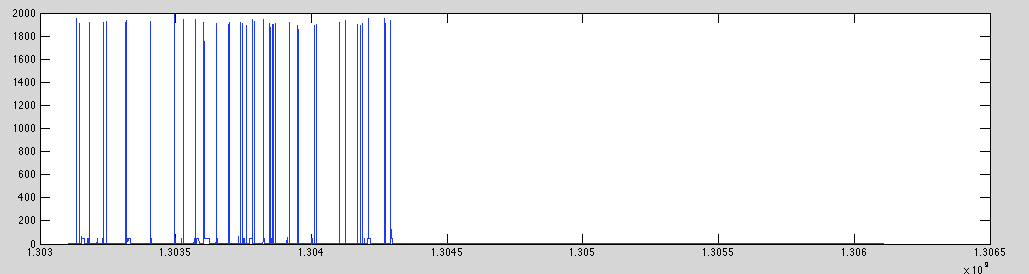
\includegraphics[width=1.0\textwidth,height=0.15\textheight]{channel_6.png}
\caption{Microwave}
\label{fig:micro}
\end{figure*}

\begin{figure*}[t]
\centering
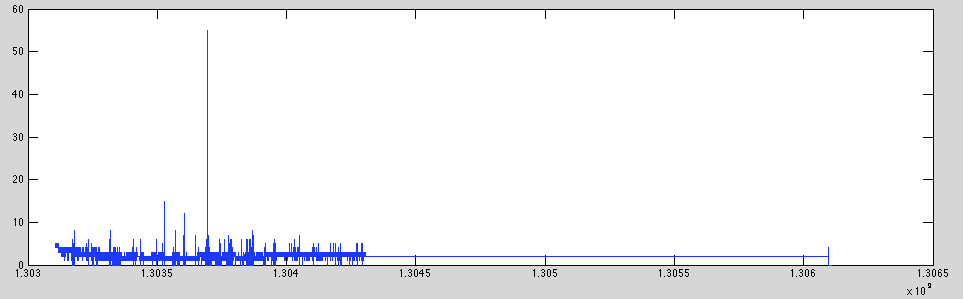
\includegraphics[width=1.0\textwidth,height=0.15\textheight]{channel_7.png}
\caption{washer\_dryer}
\label{fig:washer}
\end{figure*}

\begin{figure*}[th]
\centering
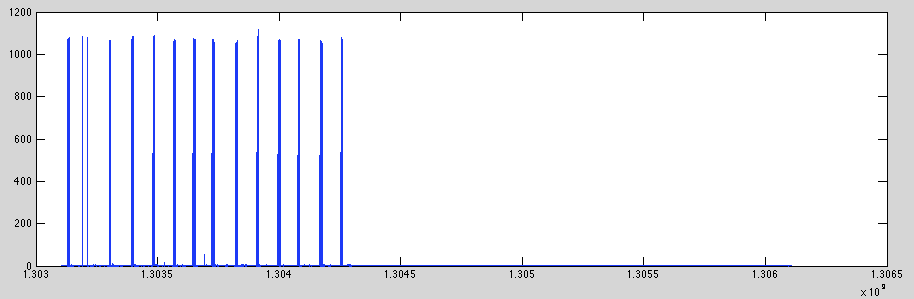
\includegraphics[width=1.0\textwidth,height=0.15\textheight]{channel_8.png}
\caption{Kitchen\_2}
\label{fig:kitchen2}
\end{figure*}

\begin{figure*}[th]
\centering
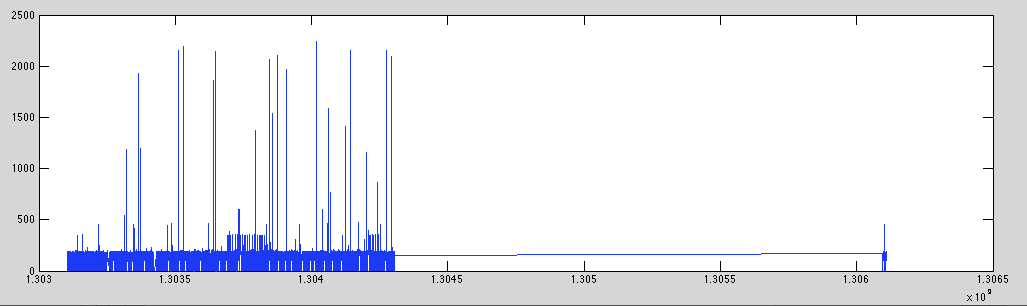
\includegraphics[width=1.0\textwidth,height=0.15\textheight]{channel_9.png}
\caption{refrigerator}
\label{fig:refri}
\end{figure*}

\item \textbf{Code } The implementation of the product of experts model is obtained from Iain Murray's website\footnote{\label{link}http://homepages.inf.ed.ac.uk/imurray2/code/}. It implements the technique described in Geoff Hinton's paper \cite{hinton2000}. 

\item \textbf{Additional details }
Some additional details regarding experiments:
\begin{enumerate}
\item The product of HMMs model (PoHMM) minimizes ``contrastive divergence" as described in the paper \cite{hinton2000}. 
\item The number of experts, $k$ used here is 15. This is set somewhat arbitrarily and needs to be experimented on.
\item Learning rate is $\epsilon = \frac{1}{300}$.
\end{enumerate}
 
\end{itemize}


%FIRST EXPERIMENT ON REDD DATASET

\subsection{Experimental Setup for REDD house 2}
Experiments are performed on the REDD which contains $9$ appliances each containing $318759$ rows of energy consumption data. Experiments are done into $4$ phases, in the first phase the number of data samples are varied corresponding to which the values of KL Divergence and convergence time are noted. In the second phase, the number of experts are varied keeping the best value of the sample from the first phase fixed. In the third phase, number of iterations are varied keeping the best values from above first two phases fixed. In the fourth part, the no. of appliances to be aggregated are varied.

\begin{table}[htdp]
\begin{center}
\begin{tabular}{| c | c | c | c |}
\hline
Samples & $KL Div$ & $T(sec)$ & $Iterations$ \\
\hline
300 & 2.4864 & 186.212 $\pm$9.087 & 18600 \\
500 & 0.6761 & 106.564 $\pm$10.046 & 10200 \\
1000 & 1.1088 & 158.521 $\pm$1.97  & 11200 \\
1500 & 3.8829 & 92.896 $\pm$8.075  & 5300 \\
2000 & 1.8686 & 130.98 $\pm$1.932 & 6900 \\
2500 & 0.4733 & 215.563 $\pm$ 2.471 & 9900 \\
3000 & 2.8204 & 258.213 $\pm1.918$ & 11000 \\
3500 & 1.2332 & 204.661 $\pm$1.713 & 7900 \\
4000 & 0.8959 & 292.666 $\pm$0.619 & 10400  \\
4500 & 1.1118 & 222.558 $\pm$1.967 & 7200  \\
8000 & 6.392 & 381.635 $\pm$2.952 & 8100  \\
10000 & 8.276 & 887.932 $\pm$13.824 & 10500  \\
15000 & 0.7201 & 1368.514 $\pm$13.605 & 9400  \\
\hline
\end{tabular}
\end{center}
\caption{Effect of varying samples on KL div and time}
\label{table: error1}
\end{table}

\begin{table}[htdp]
\begin{center}
\begin{tabular}{| c | c | c | c |}
\hline
Experts & $KL Div$ & $T(sec)$ & $Iterations$ \\
\hline
5 & 0.774 & 72.968 $\pm$1.177 & 5200 \\
10 & 1.424 & 117.482 $\pm$1.966 & 6700 \\
15 & 0.473 & 210.249 $\pm$1.258  & 9900 \\
20 & 1.56 & 217.739 $\pm$10.452 & 9000 \\
25 & 7.469 & 347.019 $\pm$8.23 & 12100 \\
30 & 2.4968 & 413.802 $\pm$7.304 & 12900 \\
35 & 1.5012 & 348.906 $\pm$14.651 & 11300 \\
\hline
\end{tabular}
\end{center}
\caption{Effect of varying experts on KL div and time}
\label{table: error2}
\end{table}


\subsection{Results}
The evaluation of how well the learning has taken place is done by using a Kullback-Leibler divergence. KL divergence of P from Q, $D_{KL}$(P$\parallel$Q) is the measure of information lost when Q is used to approximate P. Here, P is the real data and Q is a fantasy data. The two probability distributions in the REDD example refer to the expert probabilities in real and fantasy data. The learned parameters from the training are fitted to the fantasy data to measure the information lost when fantasy data is used to approximate real data.
\begin{table}[htdp]
\begin{center}
\begin{tabular}{| c | c | c | c |}
\hline
Threshold & $KL Div$ & $T(sec)$ & $Iterations$ \\
\hline
.1 & 0.473 & 210.6 $\pm$1.493 & 9900 \\
.05 & 0.443 & 240.607$\pm$2.436 & 10900 \\
.01 & 0.454 & 431.536 $\pm$14.509 & 18000 \\
.005 & 0.509 & 1167.243 $\pm$43.412 & 49800 \\
\hline
\end{tabular}
\end{center}
\caption{Effect of varying min threshold on KL div and time}
\label{table: error3}
\end{table}

\begin{table}[htdp]
\begin{center}
\begin{tabular}{| c | c | c | c |}
\hline
Appliances & $KL Div$ & $T(sec)$ & $Iterations$ \\
\hline
3 & 5.559 & 233.664 $\pm$0.579 & 10700 \\
4 & 0.188 & 465.634 $\pm$5.275 & 19900 \\
5 & .432 & 338.416 $\pm$3.988  & 13400 \\
6 & 8.736 & 606.062 $\pm$7.534 & 28100 \\
7 & 5.054 & 411.457 $\pm$10.051 & 17300 \\
8 & 0.436 & 260.544 $\pm$cc27.862 & 10700 \\
9 & 0.15 & 474.579 $\pm$14.619 & 20600 \\
\hline
\end{tabular}
\end{center}
\caption{Effect of varying appliances on KL div and time}
\label{table: error4}
\end{table}


% SECOND EXPERIMENT ON FACULTY HOUSING

\section{Proof of concept on Faculty housing data}
\label{sec:faculty}

\subsection{ Aim } To represent streams of energy consumption data from all the floors of faculty housing as a product of k HMMs. 
\subsection{Method}
\begin{itemize}
\item \textbf{ Data } This data represents the energy consumed by the IIIT Delhi faculty housing building. As a part of research, a team from IIIT Delhi has installed various temperature, light and motion sensors to perform real world studies and to analyse user preferences for energy conservation. For our analysis, we selected one month's historical data ranging from 01-01-2014, 00:01 hours to 31-01-2014, 23:59 hours. The two smart meters installed captures the data from all the floors. The first meter gives out readings from floors $0$ to $5$ and the second meter gives out readings from floors $6$ to $11$. The dataset includes timestamp and power consumed in watts and $84133$ records. Time series data from two streams are modelled as a product of $k$ HMMs. We also have the total power consumed by the faculty housing building which would serve as the ground truth to compare product of $k$ HMMs with. The data is obtained from the website whose screenshot is shown in Figure~\ref{fig:screenshot}

\begin{figure*}[t]
\centering
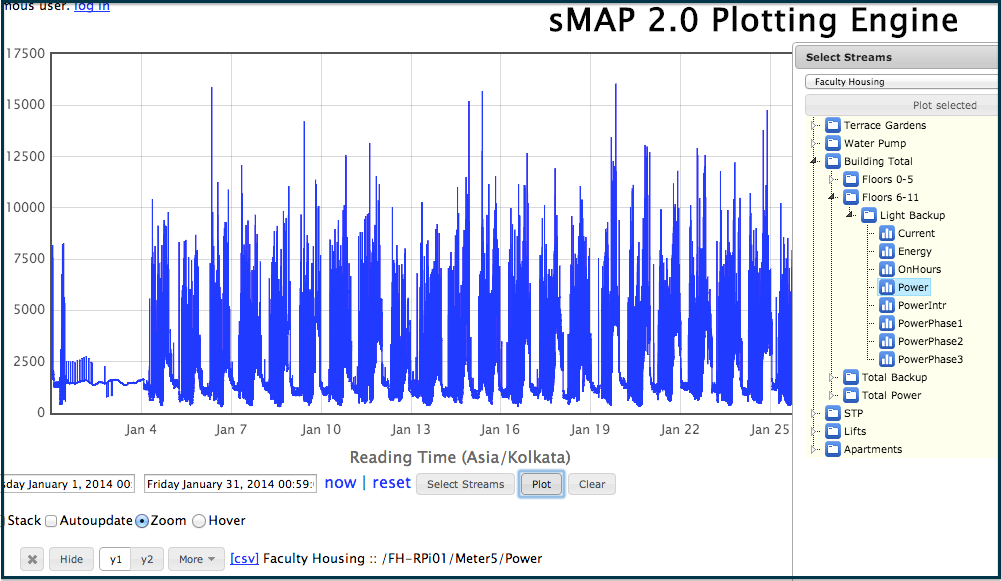
\includegraphics[width=0.8\textwidth,height=0.35\textheight]{screenshot.png}
\caption{Screen shot of the webpage}
\label{fig:screenshot}
\end{figure*}

\item \textbf{ Code } %The implementation of the product of experts model is obtained from Iain Murray's website\footnotemark[\value{http://homepages.inf.ed.ac.uk/imurray2/code/}].
It implements the technique described in Geoff Hinton's paper \cite{hinton2000}. 

\item \textbf{ Time Series :} The time series data of the energy consumption of floor 0 to 5, floor 6 to 11 and total power are plotted below in Figures~\ref{fig:flr05}, ~\ref{fig:flr611}, ~\ref{fig:total}.

\begin{figure*}[t]
\centering
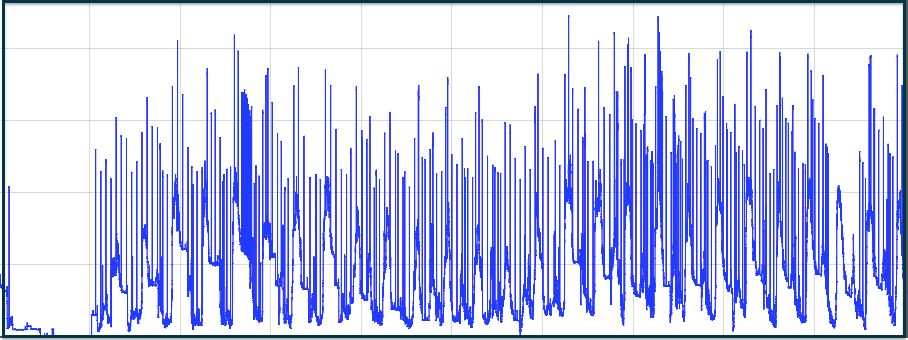
\includegraphics[width=1.0\textwidth,height=0.15\textheight]{floor052.png}
\caption{Stream 1: Power consumption of floors 0-5}
\label{fig:flr05}
\end{figure*}

\begin{figure*}[t]
\centering
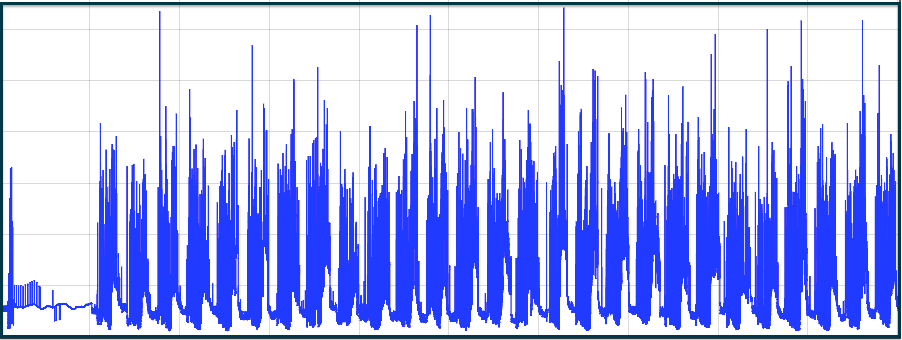
\includegraphics[width=1.0\textwidth,height=0.15\textheight]{floor6112.png}
\caption{Stream 2: Power consumption of floors 6-11}
\label{fig:flr611}
\end{figure*}

\begin{figure*}[th]
\centering
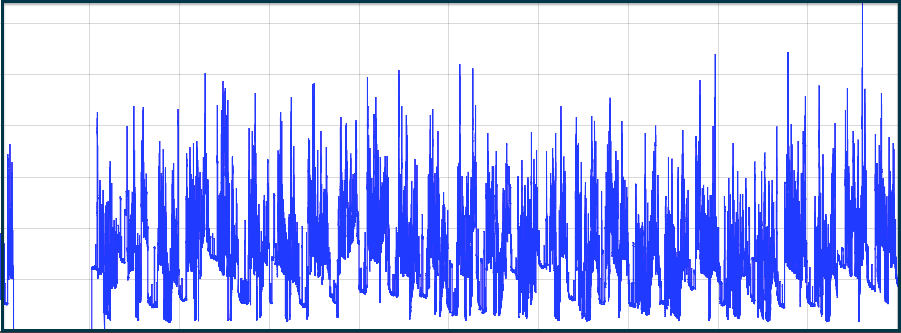
\includegraphics[width=1.0\textwidth,height=0.15\textheight]{total2.png}
\caption{Total Power of the building}
\label{fig:total}
\end{figure*}


\item \textbf{ Additional Details } 
\end{itemize}
\subsection{ Experimental Setup } 
Each of the data stream is modelled as a HMM individually. There are three streams of data, the first stream D$_{1}$ corresponds to the data from 0-5th floor, D$_{2}$ corresponds to 6-11th floor and D$_{3}$ represents the total power from the faculty housing which is represented by a fixed test set, T. Firstly, the stream D$_{1}$ is used to train the model such that the contrastive divergence is minimized. The parameters (mixing component of each unigauss, means of gaussian bits, log precisions of axis-aligned gaussian bits) that are learnt during the training are provided to the test set T in order to obtain the conditional probability of the gaussians given the data D$_{1}$ represented as pgauss$_{1}$. Similarly, the second stream of data, D$_{2}$ collected from floor 6-11, is used to learn the parameters of the model during the training phase which are then again provided to the test set T to obtain conditional probability of the gaussians given the data D$_{2}$ as pgauss$_{2}$. Finally the data D$_{3}$ is used to learn the model and parameters which are then applied to the test set T to obtain the gaussian probability as pgauss$_{3}$. Now, as we know that the total power consumption of the building should be approximately equal to the product of HMMs, which is the product of pgauss$_{1}$ and pgauss$_{2}$. If we can show that the value of pgauss$_{3}$ is as close as possible to the product of pgauss$_{1}$ and pgauss$_{2}$.\\
The experiments performed in table ~\ref{table:error5} , shows the effect of varying samples on KL Divergence, convergence time and iterations keeping minimum threshold constant at 7.\\
The other experiment performed in table ~\ref{table:error6} shows that effect of varying experts on KL Divergence and convergence time.

\subsection{ Results }
Table ~\ref{table:error5} shows that the error was minimum when the sample size was $300$. With respect to the number of experts, the error was minimum when there were $5$ experts as shown in table~\ref{table:error6}.
\begin{table}[htdp]
\begin{center}
\begin{tabular}{| c | c | c | c |}
\hline
Samples & $KL Div$ & $T(sec)$ & $Iterations$ \\
\hline
100 & 2.6219e-05 & 257 & 45100 \\
300 & 1.9753e-05 & 222 & 43200 \\
500 & 5.5493e-05 & 260 & 44800 \\
700 & 3.2847e-05 & 249 & 44000 \\
900 & 3.9486e-04 & 221 & 42600 \\
1100 & 4.9274e-04 & 317 & 44700 \\
1300 & 3.0425e-04 & 276 & 43100 \\
1500 &  3.1128e-04 & 303 & 44400\\
2000 & 1.9192e-04 & 306 & 44400\\
2500 & 1.7122e-04 & 370 & 44100 \\
3000 & 1.4686e-04 & 331 & 43300 \\
3500 & 1.2663e-04 & 370 & 43200 \\
4000 & 1.0793e-04 & 403 & 43200 \\
\hline
\end{tabular}
\end{center}
\caption{Effect of varying samples on KL div}
\label{table:error5}
\end{table}

\begin{table}[htdp]
\begin{center}
\begin{tabular}{| c | c | c |}
\hline
Experts & $KL Div (e-05)$ & $T(sec)$\\
\hline
3 & 1.9780 & 229 \\
4 & 3.5897 & 217 \\
5 & 1.9753 & 228 \\
6 & 4.3488 & 238 \\
7 & 4.9111 & 245  \\
8 & 5.6564 & 241 \\
9 & 5.4290 & 258 \\
10 & 5.5163 & 267 \\
12 & 4.4504 & 262 \\
14 & 6.9006 & 296 \\
16 & 6.8666 & 300 \\
18 & 6.2872 & 313 \\
20 & 5.3842 & 267 \\
25 & 5.8970 & 326 \\
30 & 5.9962 & 327  \\
35 & 5.2716 & 346 \\
40 & 5.0955 & 320 \\
\hline
\end{tabular}
\end{center}
\caption{Effect of varying experts on KL div and time}
\label{table:error6}
\end{table}

\section{Conclusion \& Future Work}
\label{conc}
The conclusion goes here. this is more of the conclusion




%\subsection{Length of Papers}
%
%Each accepted full paper is allocated six pages in the conference 
%proceedings, excluded references. References can take up to one page.
%Up to two additional pages may be purchased at a price 
%of \$275 per page for any accepted paper. However, all 
%{\em submissions} must 
%be a maximum of six pages, plus at most one for references, in length.
%
%
%\subsection{Word Processing Software}
%
%As detailed below, IJCAI has prepared and made available a set of
%\LaTeX{} macros and a Microsoft Word template for use in formatting
%your paper. If you are using some other word processing software (such
%as WordPerfect, etc.), please follow the format instructions given
%below and ensure that your final paper looks as much like this sample
%as possible.
%
%\section{Style and Format}
%
%\LaTeX{} and Word style files that implement these instructions
%can be retrieved electronically. (See Appendix~\ref{stylefiles} for
%instructions on how to obtain these files.)
%
%\subsection{Layout}
%
%Print manuscripts two columns to a page, in the manner in which these
%instructions are printed. The exact dimensions for pages are:
%\begin{itemize}
%\item left and right margins: .75$''$
%\item column width: 3.375$''$
%\item gap between columns: .25$''$
%\item top margin---first page: 1.375$''$
%\item top margin---other pages: .75$''$
%\item bottom margin: 1.25$''$
%\item column height---first page: 6.625$''$
%\item column height---other pages: 9$''$
%\end{itemize}
%
%All measurements assume an 8-1/2$''$ $\times$ 11$''$ page size. For
%A4-size paper, use the given top and left margins, column width,
%height, and gap, and modify the bottom and right margins as necessary.
%
%\subsection{Format of Electronic Manuscript}
%
%For the production of the electronic manuscript, you must use Adobe's
%{\em Portable Document Format} (PDF). A PDF file can be generated, for
%instance, on Unix systems using {\tt ps2pdf} or on Windows systems
%using Adobe's Distiller. There is also a website with free software
%and conversion services: {\tt http://www.ps2pdf.com/}. For reasons of
%uniformity, use of Adobe's {\em Times Roman} font is strongly suggested. In
%\LaTeX2e{}, this is accomplished by putting
%\begin{quote} 
%\mbox{\tt $\backslash$usepackage\{times\}}
%\end{quote}
%in the preamble.\footnote{You may want also to use the package {\tt
%latexsym}, which defines all symbols known from the old \LaTeX{}
%version.}
%  
%Additionally, it is of utmost importance to specify the American {\bf
%letter} format (corresponding to 8-1/2$''$ $\times$ 11$''$) when
%formatting the paper. When working with {\tt dvips}, for instance, one
%should specify {\tt -t letter}.
%
%\subsection{Title and Author Information}
%
%Center the title on the entire width of the page in a 14-point bold
%font. Below it, center the author name(s) in a 12-point bold font, and
%then center the address(es) in a 12-point regular font. Credit to a
%sponsoring agency can appear on the first page as a footnote.
%
%\subsubsection{Blind Review}
%
%In order to make blind reviewing possible, authors must omit their
%names and affiliations when submitting the paper for review. In place
%of names and affiliations, provide a list of content areas. When
%referring to one's own work, use the third person rather than the
%first person. For example, say, ``Previously,
%Gottlob~\shortcite{gottlob:nonmon} has shown that\ldots'', rather
%than, ``In our previous work~\cite{gottlob:nonmon}, we have shown
%that\ldots'' Try to avoid including any information in the body of the
%paper or references that would identify the authors or their
%institutions. Such information can be added to the final camera-ready
%version for publication.
%
%\subsection{Abstract}
%
%Place the abstract at the beginning of the first column 3$''$ from the
%top of the page, unless that does not leave enough room for the title
%and author information. Use a slightly smaller width than in the body
%of the paper. Head the abstract with ``Abstract'' centered above the
%body of the abstract in a 12-point bold font. The body of the abstract
%should be in the same font as the body of the paper.
%
%The abstract should be a concise, one-paragraph summary describing the
%general thesis and conclusion of your paper. A reader should be able
%to learn the purpose of the paper and the reason for its importance
%from the abstract. The abstract should be no more than 200 words long.
%
%\subsection{Text}
%
%The main body of the text immediately follows the abstract. Use
%10-point type in a clear, readable font with 1-point leading (10 on
%11).
%
%Indent when starting a new paragraph, except after major headings.
%
%\subsection{Headings and Sections}
%
%When necessary, headings should be used to separate major sections of
%your paper. (These instructions use many headings to demonstrate their
%appearance; your paper should have fewer headings.)
%
%\subsubsection{Section Headings}
%
%Print section headings in 12-point bold type in the style shown in
%these instructions. Leave a blank space of approximately 10 points
%above and 4 points below section headings.  Number sections with
%arabic numerals.
%
%\subsubsection{Subsection Headings}
%
%Print subsection headings in 11-point bold type. Leave a blank space
%of approximately 8 points above and 3 points below subsection
%headings. Number subsections with the section number and the
%subsection number (in arabic numerals) separated by a
%period.
%
%\subsubsection{Subsubsection Headings}
%
%Print subsubsection headings in 10-point bold type. Leave a blank
%space of approximately 6 points above subsubsection headings. Do not
%number subsubsections.
%
%\subsubsection{Special Sections}
%
%You may include an unnumbered acknowledgments section, including
%acknowledgments of help from colleagues, financial support, and
%permission to publish.
%
%Any appendices directly follow the text and look like sections, except
%that they are numbered with capital letters instead of arabic
%numerals.
%
%The references section is headed ``References,'' printed in the same
%style as a section heading but without a number. A sample list of
%references is given at the end of these instructions. Use a consistent
%format for references, such as that provided by Bib\TeX{}. The reference
%list should not include unpublished work.
%
%\subsection{Citations}
%
%Citations within the text should include the author's last name and
%the year of publication, for example~\cite{gottlob:nonmon}.  Append
%lowercase letters to the year in cases of ambiguity.  Treat multiple
%authors as in the following examples:~\cite{abelson-et-al:scheme}
%or~\cite{bgf:Lixto} (for more than two authors) and
%\cite{brachman-schmolze:kl-one} (for two authors).  If the author
%portion of a citation is obvious, omit it, e.g.,
%Nebel~\shortcite{nebel:jair-2000}.  Collapse multiple citations as
%follows:~\cite{gls:hypertrees,levesque:functional-foundations}.
%\nocite{abelson-et-al:scheme}
%\nocite{bgf:Lixto}
%\nocite{brachman-schmolze:kl-one}
%\nocite{gottlob:nonmon}
%\nocite{gls:hypertrees}
%\nocite{levesque:functional-foundations}
%\nocite{levesque:belief}
%\nocite{nebel:jair-2000}
%
%\subsection{Footnotes}
%
%Place footnotes at the bottom of the page in a 9-point font.  Refer to
%them with superscript numbers.\footnote{This is how your footnotes
%should appear.} Separate them from the text by a short
%line.\footnote{Note the line separating these footnotes from the
%text.} Avoid footnotes as much as possible; they interrupt the flow of
%the text.
%
%\section{Illustrations}
%
%Place all illustrations (figures, drawings, tables, and photographs)
%throughout the paper at the places where they are first discussed,
%rather than at the end of the paper. If placed at the bottom or top of
%a page, illustrations may run across both columns.
%
%Illustrations must be rendered electronically or scanned and placed
%directly in your document. All illustrations should be in black and
%white, as color illustrations may cause problems. Line weights should
%be 1/2-point or thicker. Avoid screens and superimposing type on
%patterns as these effects may not reproduce well.
%
%Number illustrations sequentially. Use references of the following
%form: Figure 1, Table 2, etc. Place illustration numbers and captions
%under illustrations. Leave a margin of 1/4-inch around the area
%covered by the illustration and caption.  Use 9-point type for
%captions, labels, and other text in illustrations.
%
%\section*{Acknowledgments}
%
%The preparation of these instructions and the \LaTeX{} and Bib\TeX{}
%files that implement them was supported by Schlumberger Palo Alto
%Research, AT\&T Bell Laboratories, and Morgan Kaufmann Publishers.
%Preparation of the Microsoft Word file was supported by IJCAI.  An
%early version of this document was created by Shirley Jowell and Peter
%F. Patel-Schneider.  It was subsequently modified by Jennifer
%Ballentine and Thomas Dean, Bernhard Nebel, and Daniel Pagenstecher.
%These instructions are the same as the ones for IJCAI--05, prepared by
%Kurt Steinkraus, Massachusetts Institute of Technology, Computer
%Science and Artificial Intelligence Lab.
%
%\appendix
%
%\section{\LaTeX{} and Word Style Files}\label{stylefiles}
%
%The \LaTeX{} and Word style files are available on the IJCAI--15
%website, {\tt http://www.ijcai-15.org/}.
%These style files implement the formatting instructions in this
%document.
%
%The \LaTeX{} files are {\tt ijcai15.sty} and {\tt ijcai15.tex}, and
%the Bib\TeX{} files are {\tt named.bst} and {\tt ijcai15.bib}. The
%\LaTeX{} style file is for version 2e of \LaTeX{}, and the Bib\TeX{}
%style file is for version 0.99c of Bib\TeX{} ({\em not} version
%0.98i). The {\tt ijcai15.sty} file is the same as the {\tt
%ijcai07.sty} file used for IJCAI--07.
%
%The Microsoft Word style file consists of a single file, {\tt
%ijcai15.doc}. This template is the same as the one used for
%IJCAI--07.
%
%These Microsoft Word and \LaTeX{} files contain the source of the
%present document and may serve as a formatting sample.  
%
%Further information on using these styles for the preparation of
%papers for IJCAI--15 can be obtained by contacting {\tt
%pcchair15@ijcai.org}.

%% The file named.bst is a bibliography style file for BibTeX 0.99c
\nocite{Felice,Shen,taban,Albert,wijaya2014consumer,Zhang,Daneshi,bassi,samuel,Falvo,Bakirtzis,Chen,Chow,DisaggregationHSMM,KolterJ12,KolterF11,BLTJ:BLTJ21650,Heinzelman00energy,Taylor,NYAS:NYAS5921,
Wijaya,5620917,1626400,mckerracher, benveniste,hinton2000,aistats,fhmm,andrew}


\bibliographystyle{named}
\bibliography{ijcai15}

\end{document}

